Artificial images of faces can be useful in many different applications. This includes copyright free images of people which can be used in advertising, media or anything where a face should represent a non existent person. A prime example of face generation is \url{https://thispersondoesnotexist.com/}. It uses the network SyleGAN2 introduced by \citeauthor{karras_analyzing_2020} \autocite*{karras_analyzing_2020}.\\
The approach I chose was building a DCGAN in python and training it on the CelebA\autocite{liu2015faceattributes} dataset which was not changed except a resize to $64\times 64$ pixels. 
\newpage
\subsection{Tensorflow Models}
Both models were created in the TensorFlow framework \autocite{tensorflow2015-whitepaper}. TensorFlow allowed me to create and experiment with the models in a quick manner. As described in Section~\ref{ref:vanilla_gan}, a generator and a discriminator model is needed. 

\subsubsection{The Generator Model}
\label{ref:faces_dcgan_gen}
The Generator uses a latent vector with the shape $n_z=128$ to provide enough input variance as input. The input layer is connected to a \gls{dense} with $4 \cdot 4 \cdot 256$ or $4096$ neurons and a ReLU activation function. To continue in a convolutional fashion, the vector outputted by the fully connected layer needs to be reshaped into a three dimensional matrix of shape $4\times 4\times 256$. The \gls{dropout} with a probability of 20\% prevents mode collapse, since the generator is not able to become too adjusted to the current iterations discriminator.
This layer is followed by 4 sets of transpose, leaky ReLU and batch normalisation layers. The transpose layers have a filter size of $2\times 2$, a stride of 2. 
The first Transpose layer or $n=0$ has 256, the second layer $n=1$ has 128 filter. Generally speaking the filter amount is determined by $\frac{256}{n\cdot 2}$
The output layer of the generator is a convolutional layer with a filter amount of 3, a filter size of $1\times 1$, a stride of 1 and the tanh activation function so that the Generator produces normalized image data. \\
The Generator plot can be seen in Figure~\ref{apx:dcgan_generator}.

\subsubsection{The Discriminator}
The Discriminator's input has the shape $64\times 64\times 3$, since this is the shape of the images in the dataset. Following this layer is a convolutional layer with 8 filters, each with a size of $3\times 3$ and no stride, an average \gls{pooling} layer and a leaky ReLU layer with $\alpha = 0.02$. These three layers get repeated three times, with the amount of filters increasing by a factor of 2. The first set of layers out of this collection has in addition a batch normalisation layer. The second has a additional \gls{dropout} with a dropout chance of 30\%. The last set has no additional layers but is followed by a flatten layer to convert the three dimensional matrix into a vector. The vector gets passed through a \gls{dropout} (30\% Dropout probability) into a \gls{dense} with 32 neurons followed by the output layer with one neuron.\\
A plot of the Discriminator can be seen in Figure~\ref{apx:dcgan_discriminator}.

\subsection{The training Loop}
\begin{minted}
[
frame=lines,
framesep=2mm,
baselinestretch=1.2,
bgcolor=LightGray,
fontsize=\footnotesize,
linenos
]
{python}
for i in range(self.d_steps):
    latent_vector = tf.random.normal(shape=(batch_size, self.latent_dim))
    with tf.GradientTape() as gt:
        generated_images = self.generator(latent_vector, training=True)
        prediction_fake = self.discriminator(generated_images, training=True)
        
        flipped_images = tf.image.random_flip_left_right(images)
        prediction_real = self.discriminator(flipped_images, training=True)
        
        d_loss = self.d_loss_fn(prediction_real, prediction_fake)
    d_gradients = gt.gradient(d_loss, self.discriminator.trainable_variables)
    self.d_optimizer.apply_gradients(zip(d_gradients, self.discriminator.trainable_variables))
\end{minted}
\captionof{listing}{Discriminator training loop}
\label{code:disc_train_loop}
The training loop was written using a class extending \texttt{keras.Model} and overwriting the \texttt{train\_step()} function so that I could use the \texttt{model.fit()} function and additional tools provided by TensorFlow like TensorBoard for measuring progress and callbacks to save images and checkpoints while training. \\
The discriminator training step can get repeated multiple times if needed. In the current version of the model, this is not needed, since the discriminator slowly converges. Each time a latent vector for the generator with the shape $batch\_size \times 128$ is generated using the \texttt{tf.random.normal()} function. This vector is passed into the generator producing a vector of images which are evaluated by the discriminator. To limit the change of the discriminator \gls{overfitting} and to introduce more variety, the training images get randomly flipped using the function \texttt{tf.image.random\_flip\_left\_right()} before being judged by $D$. The code for the discriminator training loop can be seen in Source Code~\ref{code:disc_train_loop}.
\\
The Generator train step is as describes in Section~\ref{ref:GAN_training}.\\
The loss is calculated as seen in Source Code~\ref{code:loss_functions}. It is important to note, that the binary crossentropy function has the \texttt{from\_logits} attribute set to true, so that the logits produced by the Discriminator can be used for cross entropy loss.\footnote{More on cross entropy loss can be read in Section~\ref{ref:binary_crossentropy}.} The function \texttt{discriminator\_loss(real\_output, fake\_output)} calculates $BCECost(1, O_{D(x)}) + BCECost(0, O_{D(G(z))})$. In the same code example it is also visible that the Adam optimizer with a learning rate of $1e-4$ is used for both $D$ and $G$. 

\begin{minted}
[
frame=lines,
framesep=2mm,
baselinestretch=1.2,
bgcolor=LightGray,
fontsize=\footnotesize,
linenos
]
{python}
cross_entropy = keras.losses.BinaryCrossentropy(from_logits=True)
def discriminator_loss(real_output, fake_output):
    real_loss = cross_entropy(tf.ones_like(real_output), real_output)
    fake_loss = cross_entropy(tf.zeros_like(fake_output), fake_output)
    total_loss = real_loss + fake_loss
    return total_loss

def generator_loss(fake_output):
    return cross_entropy(tf.ones_like(fake_output), fake_output)

generator_optimizer = tf.keras.optimizers.Adam(1e-4)
discriminator_optimizer = tf.keras.optimizers.Adam(1e-4)
\end{minted}
\captionof{listing}{custom loss functions for both $D$ and $G$}
\label{code:loss_functions}

\subsection{Problems while training}
Many training iterations failed due to mode collapse. To counter this I tried adding noise to the data passed into the Discriminator to decrease the chance of \gls{overfitting}. This however did not help as much increasing the length of the latent vector and removing some complexity from the generator.\\
Another problem was that the Discriminator learned too fast to distinguish the images and thus giving the Generator no meaningful feedback. Fortunately, since the loss of $D$ rapidly approaches zero, this issue can be identified early enough to avoid spending too much time training a model that is destined to fail. This time, reducing the filters by $\frac{1}{4}$ in all convolutional layers of $D$ resolved the problem. 

\subsection{Importing the Model into Matlab}
\begin{figure}
    \centering
    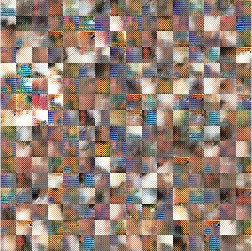
\includegraphics[width=0.5\textwidth]{images/rubbishImport_cropped.jpg}
    \caption{16 generated Images using imported model}
    \label{fig:rubbishImport}
\end{figure}
The model can be imported into Matlab by using the \texttt{importKerasLayers} function. It is important to also load the weights of the model, else model has to be trained again.\\
An additional step which has to be taken when using my generator is to replace the \texttt{tf.keras.layer.Reshape} layer with a custom function layer, since Matlab does have its own corresponding layer.
\begin{minted}
[
frame=lines,
framesep=2mm,
baselinestretch=1.2,
bgcolor=LightGray,
fontsize=\footnotesize,
linenos
]
{matlab}
layers = importKerasLayers("generator_model/generator.h5", "ImportWeights",true);

reshape_layer = functionLayer(@(x) dlarray(reshape(x, 4,4,256, []), "SSCB"), ...
                Formattable=true, Acceleratable=true);

layers_new = replaceLayer(layers, "reshape_1", reshape_layer);
generator = dlnetwork(layers_new);
\end{minted}
\captionof{listing}{Code to import the Generator}
\label{code:import_gen}
Although I was able to import the model, Matlab had problems interpreting the weights, giving me useless results like in figure~\ref{fig:rubbishImport}

\subsection{Results}
\begin{figure}[H]
    \centering
    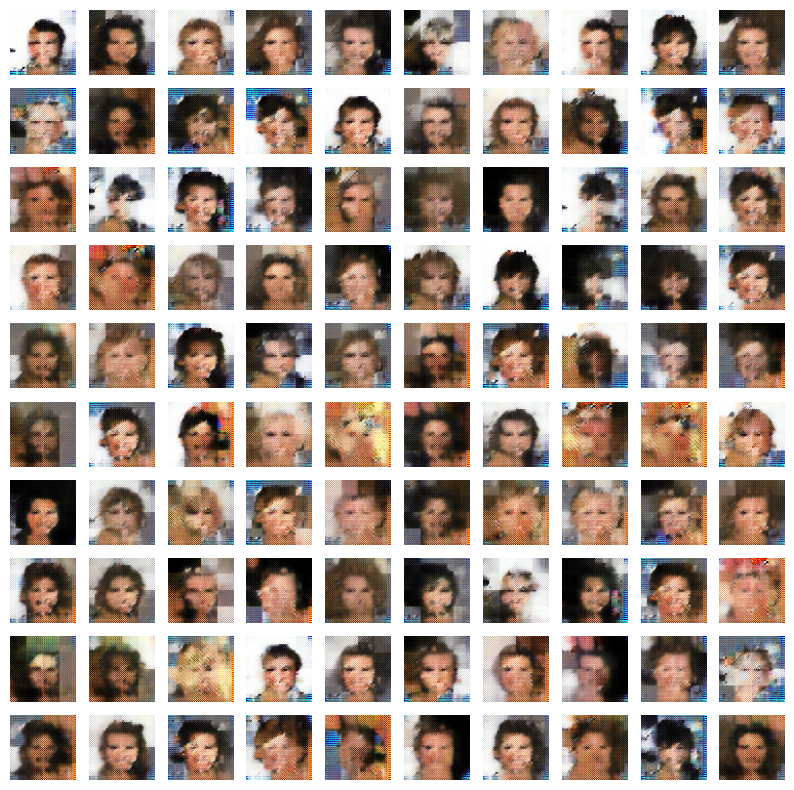
\includegraphics[width=0.7\textwidth]{images/faces.png}
    \caption{100 artificial faces}
    \label{fig:faces_dcgan}
\end{figure}
The images visible in figure~\ref{fig:faces_dcgan} were generated by the model described in section~\ref{ref:faces_dcgan_gen}. This Generator was trained for 455 Iterations. More Images can be generated using the script~\ref{apx:generation_code}.
This model has clearly some flaws. First of all, the image quality is not great. Some faces are not recognizable, others consist mostly out of black pixels. To improve this the generator network needs to be refined and more training epochs are needed. Second the images suffer from the check board pattern associated with transposed convolutions. More on how to prevent this effect can be read about in section~\ref{ref:image_quality}.\\
Implementing the aforementioned changes, the image quality could be greatly improved.\\
Additional Images generated during training can be found on the USB-Stick or at \url{https://github.com/SFSeeger/w-seminar}. The code is also available in the appendix: \ref{apx:celebGAN}.

\subsection{celebGAN2}
CelebGAN2 is a project which I made to improve image Quality of the first model. I was not planning on showing it, since it was training while writing this paper and not producing any results showing improvement. This changed however as soon as i saw this paper as completed. \\
This GAN was trained in 319 iterations. Both the generator and Discriminator Loss can be found in the appendix in section~\ref{apx:celebGAN2Loss}.
\subsubsection{Changes}
Changes were only done to the generator. These changes are moving the Batch normalisation layer before the leaky ReLU layer and changing the last convolution layer to use a kernel size of $4\times4$ and zero-padding. 
\subsubsection{Results}
\begin{figure}[H]
    \centering
    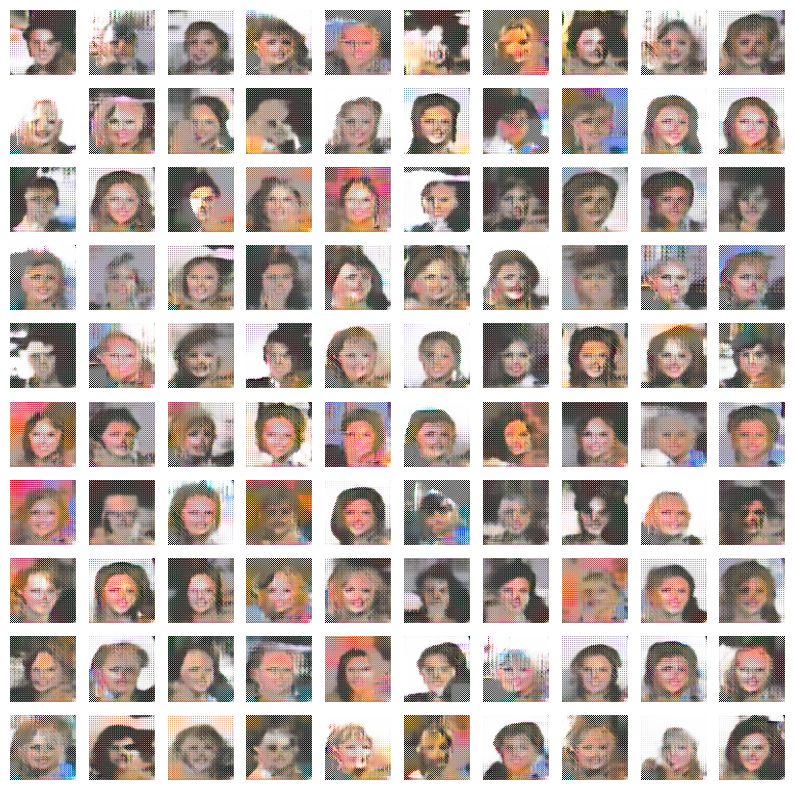
\includegraphics[width=0.7\textwidth]{images/faces2.png}
    \caption{100 Images of celebGAN2}
    \label{fig:pred_celebGAN2}
\end{figure}
The Results are visible in Figure~\ref{fig:pred_celebGAN2}. As shown the faces are better recognisable than in Figure~\ref{fig:faces_dcgan} which is promising. But this model still has some issues. First, the Images are less saturated and vibrant as the images produced by the first version of the model and the checkboard effect is still visible. In addition is the background stronger blurred. The code is available in the appendix: \ref{apx:celebGAN2}.